\documentclass[]{article}
\usepackage[brazil]{babel}
\usepackage[utf8]{inputenc}
\usepackage{amsmath,amssymb,amsfonts,textcomp}
\usepackage{graphicx}
\usepackage{float,flafter}
\usepackage{hyperref}
\usepackage{inputenc}

\usepackage{enumerate}
\usepackage{alltt}
\linespread{1.1}
\usepackage{listings}
%opening
\title{Otimização de Lanchas do SAMU utilizando Algoritmo Genético Multiobjetivo}
\author{Luiz Eduardo Fernandes Bentes}

\begin{document}

\maketitle

\begin{abstract}

\end{abstract}

\section{Descrição do método}
A geometria de um casco com apenas uma linha de chine pode ser definida pelas linhas de "chine", "sheer" e linha central. Este tipo de casco possuiu uma proa plana e pode ser modelada pela decomposição da superfície em limites ou curvas de controle que serão restringidas pelos parâmetros de projeto.

Esses parâmetros numéricos incluem \textbf{posição} e \textbf{inclinação}. No caso do chine, que é a curva mais significativa de um projeto de casco de planeio, a área fechada (Ac) e centróide (XC) também estão incluídos nos parâmetros numéricos. As curvas de fronteira são a \textbf{quilha ou linha central (CL)}, a \textbf{linha de chine} e a linha pura. O objetivo do método apresentado é criar superfícies de B-spline para representar um casco de navio com base nas restrições mostradas na Tabela 1 com o significado gráfico mostrado na Fig. 2. 

Os parâmetros na Tabela 1 têm o significado gráfico representado na Fig. 2, onde os vetores indicam o ângulo entre o eixo X e a linha da seta.

\begin{table}[th]
	\centering
	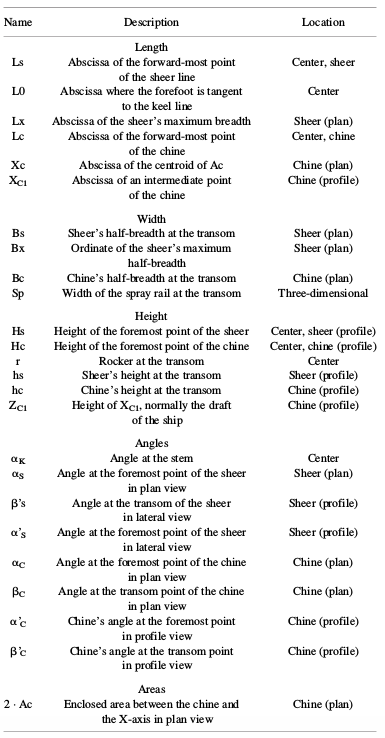
\includegraphics[width=0.67\linewidth]{parametros}
	\caption{Parâmetros da construção do casco da embarcação}
	\label{fig:parametros}
\end{table}


Os parâmetros selecionados usados para definir estas curvas tem significado para o projetista e pode ser relacionado com futuros aspectos do design da embarcação.A definição da curva foi simplificada ao considerar que o casco possui uma ~travessa~ vertical plana e que o ponto posterior de todas as curvas tem uma abscissa zero como na Fig. 2

No caso da travessa não-vertical (nonvertical transom), a definição pode ser facilmente reconfigurada considerando uma abscissa diferente de zero para os pontos acima mencionados, que será uma função do ângulo da trave.

Uma característica de design muito importante, o angulo de deadrise da travessa, $\Omega$, é derivada de \textit{hr}, \textit{hc} e \textit{Bc}, $\Omega = \text{Arctan}\left(\dfrac{h_c - h_r}{B_c}\right).\left(\dfrac{180}{\pi}\right)$


As dimensões máximas globais do comprimento e largura do casco são Ls e 2 Bx, respectivamente. O método permite a definição de um trilho de pulverização de uma determinada largura, Sp, ao longo do chine.

O método é dividido em dois domínios diferentes: acima e abaixo da curva de chine. O método controla a concavidade/convexidade das curvas utilizando um parâmetro que controla o desvio máximo de cada parte até o segmento reto.

\subsection{B-spline}

Para introduzir a notação para este artigo, um curto resumo de B-splines segue-se. Uma curva B-spline é formada por diversas partes de curvas polinomiais, chamadas de partes Bézier, e a curva completa é $C^2$ (Curvatura comum ou segunda derivada) nas junções no caso das B-splines cúbicas. A curva é definida com um polígono, chamado polígono controle, e com a ajuda de um algoritmo de interpolação que permite a construção relacionando a curva com o polígono 

As etapas de interpolação são codificadas em uma família de funções polinomiais por partes, $B_j^n(u)$, chamadas funções B-spline do n-ésimo grau, e são calculadas usando o algoritmo de De Boor. As B-splines cúbicas são as curvas mais utilizadas no design de navios e aquelas que geralmente se encaixam melhor nas splines tradicionais do loftsman.


\end{document}
